\documentclass[border=4pt]{standalone}
\usepackage{tikz}
\usetikzlibrary{decorations.pathmorphing}
\begin{document}
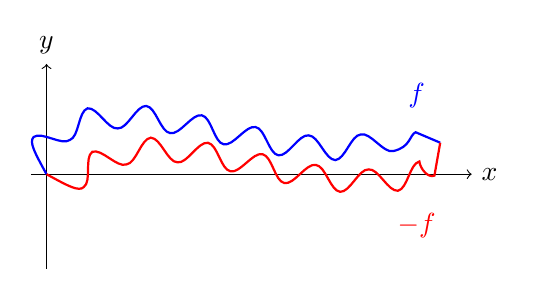
\begin{tikzpicture}
  \draw[->] (-.2,0) -- (5.4,0) node[right] {$x$};
  \draw[->] (0,-1.2) -- (0,1.4) node[above] {$y$};
  \draw[blue,thick,decorate,decoration={snake,segment length=7mm,amplitude=1.5mm,raise=3mm}]
    (0,0) .. controls (1.2,1.2) and (3.4,-.8) .. (5,.4);
  \draw[red,thick,decorate,decoration={snake,segment length=7mm,amplitude=1.5mm,mirror,raise=3mm}]
    (0,0) .. controls (1.2,1.2) and (3.4,-.8) .. (5,.4);
  \node[blue] at (4.7,1) {$f$};
  \node[red] at (4.7,-.65) {$-f$};
\end{tikzpicture}
\end{document}
